\newChapter{The Acquire and Process Description Language Ecosystem}{chap:apdl_ecosystem}

\section{Introduction}
\label{sec:apdl_ecosystem_intro}

The APDL ecosystem is the work done around the compiler in order to validate the
project. We will show the implementation of the serial handler and some example,
so the user will be able to create his own handler if he wants.

Then, we will show the storage and the visualisation of the data. The
technologies used for this part are recent and completely free.

Finally, we will implement, from scratch, an \gls{APDL} system and show how to
launch the generated entity one by one.

\section{The Serial Handler}
\label{sec:serial_handler}

The \gls{APDL} \gls{DSL} don't go further than the serial network. The system
only receives, process and sends the data through a serial with a certain
format. After that, \gls{APDL} don't know what happens to the data.

A very simple serial handler has been developed using the Python language. Python
offers a library called ``pyserial'' which simplify the handling of serial
connections. The listing \ref{lst:serial_handler_python} shows the very simple
implementation of a serial handler using Python.

\begin{listing}[H]
  \centering
\begin{pythoncode}
import serial
arduino = serial.Serial('/dev/ttyACM0', 9600, bytesize=8, timeout=1)

data = arduino.readLine()
asciiData = data.decode('ascii')

# format of data = "topic : value"
array = asciiData.split(":")
topic: str = array[0]
value: str = array[1]

# replace the \n from the device
value = value.replace("\n","",1)
value = value.replace("\r","",1)
\end{pythoncode}
  \caption[Simple serial handler implementation in Python]{Simple serial handler
implementation in Python. Pyserial simplifies the recovering process and the
Python standard library offers some functions to decode the data.}
  \label{lst:serial_handler_python}
\end{listing}

Once the data has been recovered, the user can do anything he wants with it. For
example, the \gls{APDL} handler implemented as part of this project is sending
the data to an InfluxDB database\cite{InfluxData}.

APDL offers the possibility to automaticaly generate an handler implementation
in python with the corresponding identifier. This possibility is activated by
using the option ``--generate-handler'' with the \gls{APDL} compiler. Otherwise,
the user could define his own handler.

\begin{listing}[ht]
  \centering
\begin{pythoncode}
import serial

from datetime import datetime
from influxdb import InfluxDBClient


def main():
    arduino = serial.Serial('/dev/ttyACM0', 9600, bytesize=8, timeout=1)

    user = 'root'
    password = 'root'
    dbname = 'apdl-default'

    client = InfluxDBClient('localhost', 8086, user, password, dbname)
    client.drop_database(dbname)
    print("Create database")
    client.create_database(dbname)

    # The format is
    # topic : value

    while True:
        data = arduino.readline()
        asciiData: str = data.decode('ascii')
        try:
            array = asciiData.split(":")
            topic: str = array[0]
            value: str = array[1]
            value = value.replace("\n", "", 1)
            value = value.replace("\r", "", 1)
            value = value.replace(" ", "")
            topic = topic.replace(" ", "")
            if "temp" not in topic:
                continue
            print("Send to influxdb == " + topic + " : " + value)
            json = [
                {
                    "measurement": topic,
                    "fields": {
                        "value": int(value)
                    }
                }
            ]
            client.write_points(json)
        except IndexError:
            continue
        except serial.serialutil.SerialException:
            continue

if __name__ == "__main__":
    main()
\end{pythoncode}
  \caption[Example of an APDL Serial Handler with InfluxDB]{Example of an
\gls{APDL} Handler which is also working with InfluxDB. The data are recovered
from the serial connection and send to InfluxDB.}
  \label{lst:handler_python_example}
\end{listing}

Listing~\ref{lst:handler_python_example} shows an implementation of an
\gls{APDL} handler. The implementation is very small and allow the user to
completly modify as much as he wants.

\section{Data Storage and Visualisation}
\label{sec:data_storage}

The \gls{APDL} compiler also produce a Docker-compose configuration file. This
configuration file allows a simple ecosystem generation by using Docker. In order
to store the data acquired by the device and to visualise them, we used two
products : InfluxDB and Grafana.

InfluxDB\cite{InfluxData} is a real-time database focused on time series. The
data we aquire through \gls{APDL} could be seen as time series, so InfluxDB is
perfect for this kind of project.

Grafana\cite{GrafanaLabs} is an open plaform for data analytics, monitoring and
visualisation. The tool is provided with an automatic connection to InfluxDB.
Figure \ref{fig:grafana_example} shows Grafana in action, we can see a graph
representation of the temperature values recovered by an \gls{APDL} device.

\begin{figure}[ht]
  \centering
  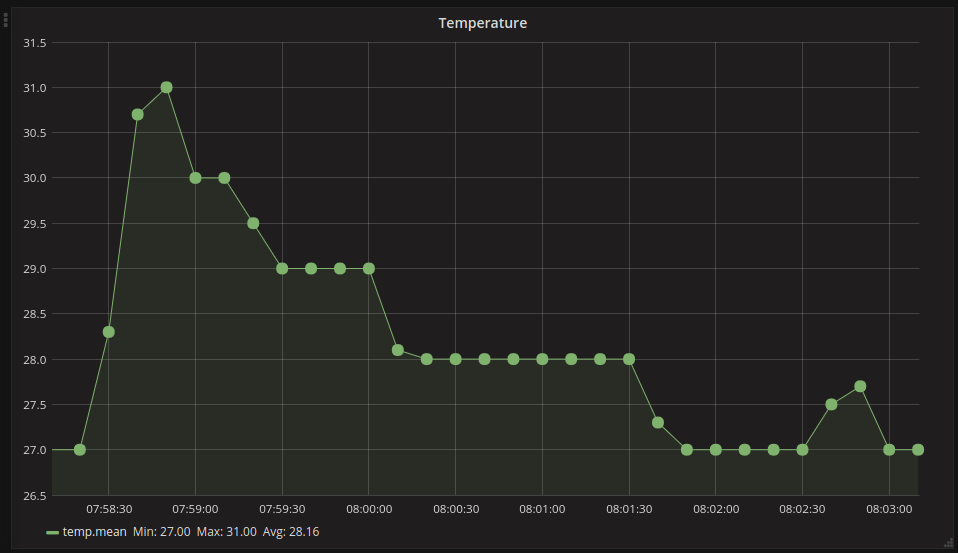
\includegraphics[width=0.9\textwidth]{img/grafana_example}
  \caption[Visualisation of the temperature using Grafana]{Visualisation of the
    temperature acquired by an \gls{APDL} device. The visualisation is done by
    using Grafana, a free plaform for data analytics, monitoring and visualisation.}
  \label{fig:grafana_example} 
\end{figure}

Unfortunately, current \gls{APDL} compiler does not provide an immediate way of
visualising the data. When we launch the project for the first time, the Grafana
image is pull by docker and the user needs to configure the visualisation by
himself.

\section{A Complete Example}
\label{sec:a_complete_example}

As an example, we will show a complete development of an APDL project from the
start to the end. The goal is to build a simple system to visualise the
temperature of the room. The chosen device is the Arduino
UNO~\cite{Store2014}. The figure~\ref{fig:demo_device} shows the installation of
the device with a temperature sensor.

\begin{figure}[ht]
  \centering
  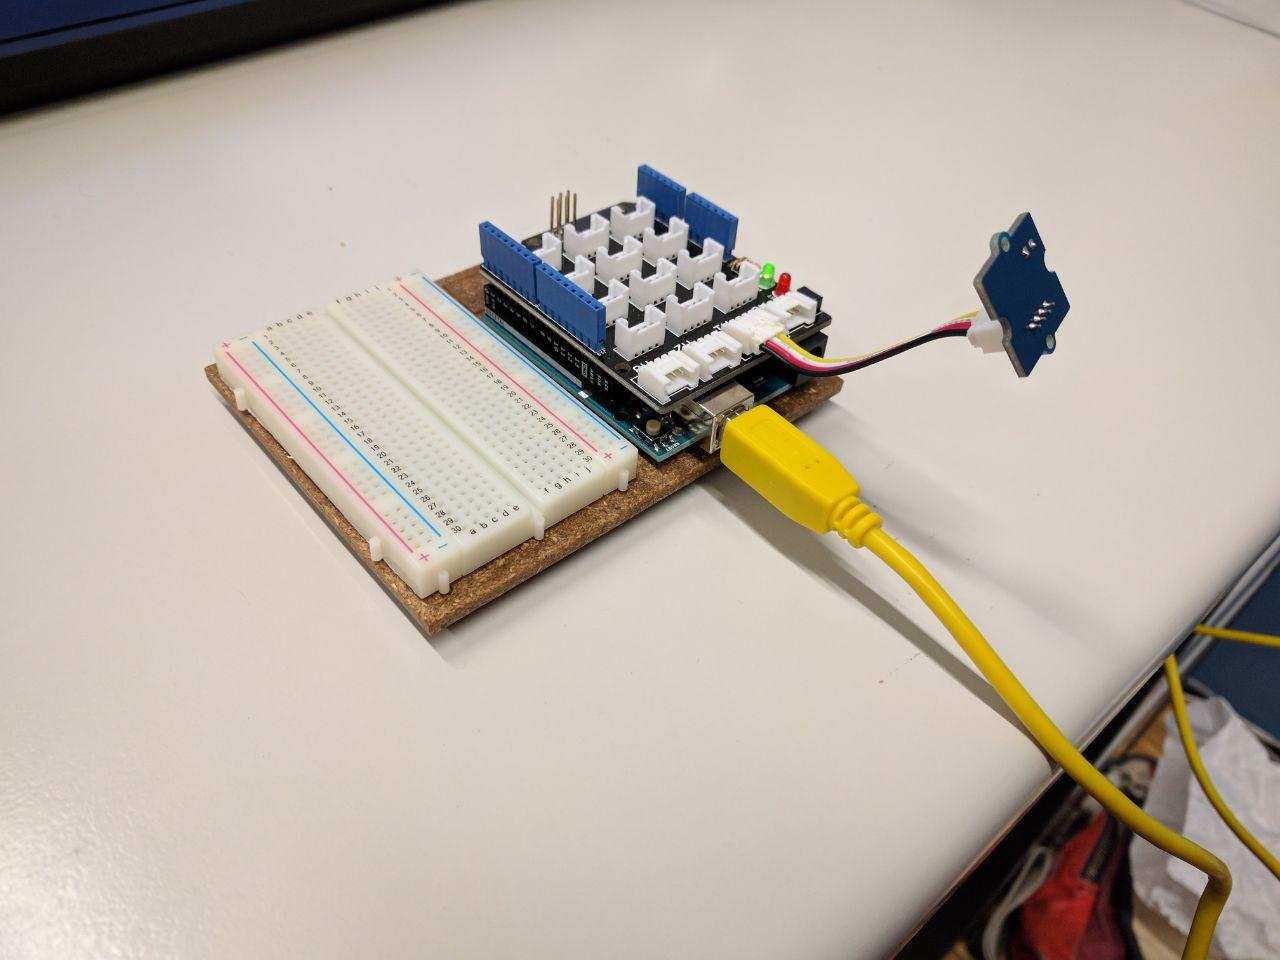
\includegraphics[width=0.60\textwidth]{img/demo_device}
  \caption[Device instalation of the complete example]{Device installation of
    the complete example. We just use a temperature sensor connected to the pin
    ``A1'' of the Arduino.}
  \label{fig:demo_device} 
\end{figure}

Now we will write the code of our corresponding system. The
listing~\ref{lst:demo_code} shows the implementation, with APDL, of the project.
Firstly, we define the name of the project and includes a file named
``apdl\_component.apdl''. This file, available in appendix
\ref{app:apdl_component_apdl}, provides the analog and digital inputs definition
for Mbed and Arduino. Then, we can declare our device with the corresponding
inputs and serials. Finally, we define a transformation function named ``tf''.
The temperature sensor on the arduino give back the value of the resistance. So
we need to compute the temperature with this value.

\begin{listing}[H]
  \centering
\begin{apdlcode}
project_name = "Example"

@include "apdl_component.apdl"

@device arduino1 {
    id = uno
    framework = arduino
    @input t analogInput 1
    @input temp tf t
    @serial temp each 1 s
}

@define transform def tf (x:int) -> float {
    val B : int = 3975
    val resistance : float = (float)(1023 - x) * 1000 / x
    val temperature : float = 1 / (log(resistance/1000) / B + 1 / 298.15) - 273.15
    return temperature
}
\end{apdlcode}
  \caption[APDL implementation of the complete example]{APDL implementation of
the complete example. We declare a device with the id ``uno'' and the framework
``arduino'' then we import the file ``apdl\_component.apdl'' which provides some
inputs. Finally, we define the transformation function ``tf'' using the \gls{TF}
language, as well as the inputs and the serial.}
  \label{lst:demo_code}
\end{listing}

Once we are compiling the project, the compiler generates a directory with all
the necessary entities to launch the project. The generated bash script executes
the following commands :

\begin{minted}{bash}
# upload the code to the device
platformio run -t upload
# launch the docker images for influxdb and grafana
docker-compose up
# launch the serial handler and start sending the data to influxdb
python handler.py
\end{minted}

Now, we can visualise the temperature of the room with Grafana. For that, we open a
browser and write ``localhost:3000''. Now we can look at the room's temperature.
First, we have to configure a data source with a direct connection to influxdb.
The identifier and password for the administator access are ``root''. Finally,
we have to create a Dashboard, select the corresponding points in influxdb and
that's all.

Further work is planned in order to fully automated the \gls{APDL} compilation
process so that the user has the minimal set of action to do.

\section{Summary}
\label{sec:apdl_ecosystem_summary}

The work done around the APDL compiler is simple and easely reproducible. We saw
the implementation of the APDL's handler and how the user can modify it for
personal purposes.

We also documented the storage and visualisation of the data. Both used
technologies, InfluxDB and Grafana, are free and very easy to use even for
people whose knowledge is basic.

Finally, we saw a complete example of an APDL project implemented from scratch
and the its results. Not all the part are fully automated but further work are
planned to do so.

%%% Local Variables:
%%% mode: latex
%%% TeX-master: "../thesis"
%%% End: